\chapter{Introduction}

Here is the introduction.
It's where you talk about your study and how cool it is.
If you want to cite someone, you can do it like this \cite{preston1999}.
Of course, if you want to cite \citeA{preston1986}, you'd do it like this.
Check out the APAcite documentation if you need to cite things in another way.

\section{A new section}

In this section, I'll insert a figure. 
Figure \ref{fig:koala} shows a koala in the rain.

\begin{figure}[b!]
\centering
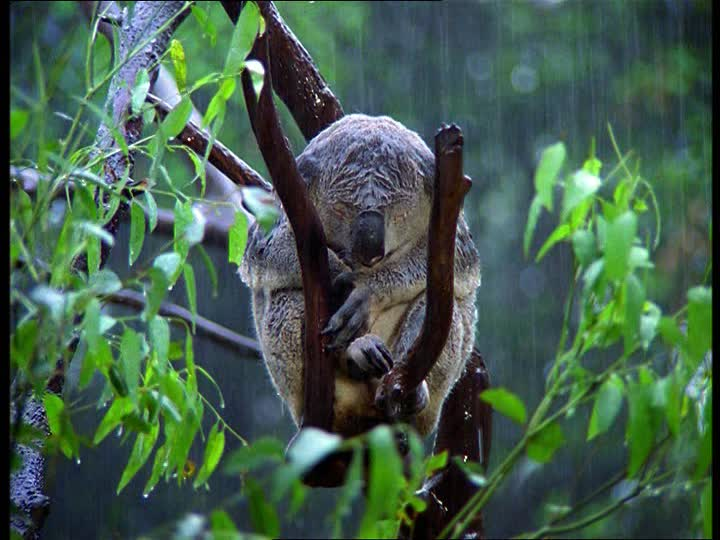
\includegraphics[width=1\textwidth]{koala}
\caption{This is a koala in the rain}
\label{fig:koala}
\end{figure}

To paraphrase Ze Frank, this koala evidences an abundance of apathy regarding its situation.

\subsection{A subsection}

Sometimes it is useful to have two images as part of the same figure.
Figure \ref{fig:unlikelyEvents} shows a cat (briefly) being sweet to a dog and a location that Kramer refers to as the ``nexus of the universe.''

\begin{figure}[ht!]
\centering
\subfloat[]{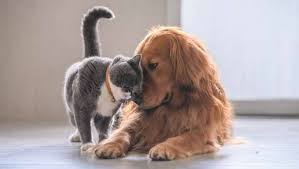
\includegraphics[width=0.45\textwidth]{dogAndCat}}
\subfloat[]{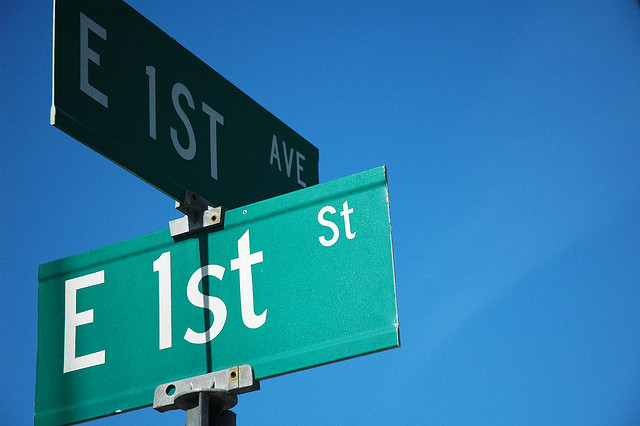
\includegraphics[width=0.45\textwidth]{nexusOfUniverse}}
\caption{Examples of inauspicious events.}
\label{fig:unlikelyEvents}
\end{figure}	